\section{Metaheuristieken}
\label{s:metaheuristics}
\chapterquote{Ik heb geen oplossing, maar ik bewonder het probleem.}{Anthelme Brillat Savarin, Frans politicus en advocaat (1755-1826)}
Een tak van de Arificiële Intelligentie die zich vooral bezighoudt met optimalisatieproblemen is de \termen{Metaheuristiek} (niet te verwarren met Heuristieken bij zoeken). Optimalisatieproblemen zoals bijvoorbeeld het \termen{Traveling Salesman Problem (TSP)}, het \termen{Knapsack Problem}, enzovoort. Hierbij is het niet de bedoeling dat we een oplossing vinden (zoals in de voorgaande secties eerder het geval was). Maar waarbij we dynamisch tussen oplossingen kunnen wisselen, en waar we op zoek zijn naar een oplossing die één of meerdere parameters optimaliseert. Problemen die moeilijk te implementeren constraints op de oplossing opleggen zijn dus beter te vermijden. Typisch  zal een Metaheuristiek dit probleem proberen op te lossen in een polynomiale tijd. Terwijl de problemen meestal een exponentieel gedrag kennen, indien we de optimale oplossing willen kennen. Bijgevolg zal een Metaheuristiek niet altijd de meest optimale oplossing vinden, maar meestal een acceptabele oplossing in ruil voor een realistische rekentijd.
\paragraph{}
Algemeen kunnen we dus stellen dat Metaheuristieken hoofdzakelijk bedoeld zijn om \termen{NP-Complete Problemen} op een redelijke manier op te lossen in min of meer constante tijd (de meeste Metaheuristieken zullen immers na een bepaalde tijd meestal niet meer met betere resultaten komen). Verder hebben de meeste Metaheuristieken een toevalscomponent, dit \termen{Stochastisch gedrag} resulteert over het algemeen in een beter en sneller resultaat. In tegenstelling tot deterministische heuristieken die af en toe in vallen kunnen terechtkomen waar ze niet uitgeraken. Metaheuristieken zijn ten slotte ook algemeen en niet probleem-specifiek. De meeste Metaheuristieken vragen een functie die de \termen{Utility-waarde} van een oplossing weergeeft een eventueel een set aan constraints waaraan een oplossing hoort te voldoen.
\paragraph{}Hoewel het concept nog behoorlijk recent is (De term ``Metaheuristiek'' duikt voor het eerst op in 1986), bestaan er tientallen verschillende technieken. Metaheuristieken aan zich zijn dan ook eerder een ``Framework'' of een set van ontwerp richtlijnen voor het oplossen van een probleem. De meeste van deze Metaheuristieken zijn bovendien gebaseerd op fenomenen uit de Natuurkunde, Biologie, Wiskunde of Scheikunde. Hieronder een beperkte lijst met metaheuristieken:
\begin{multicols}{2}
\begin{itemize}
 \item \termen{Genetische Algoritmen} (zie \ref{ss:geneticAlgorithms} op pagina \pageref{ss:geneticAlgorithms})
 \item \termen{Evolutionary Algoritms}
 \item \termen{Tabu Search} (zie \ref{ss:tabuSearch} op pagina \pageref{ss:tabuSearch})
 \item \termen{Simulated Annealing} (zie \ref{ss:simulatedAnnealing} op pagina \pageref{ss:simulatedAnnealing})
 \item \termen{Great Deluge}
 \item \termen{Hyperheuristics} (zie \ref{ss:hyperheuristics} op pagina \pageref{ss:hyperheuristics})
 \item \termen{Variable Neighbourhood Search} (zie \ref{ss:variableNeighbourhoodSearch} op pagina \pageref{ss:variableNeighbourhoodSearch})
 \item \termen{Late Acceptance}
 \item \termen{Extreme Optimisation}
 \item \termen{Neural Networks}
 \item \termen{Electrostatic Potential}
\end{itemize}
\end{multicols}
\subsection{Leidend Voorbeeld: Het binair knapzakprobleem}
\begin{leftbar}
Als illustrerend voorbeeld kiezen we voor het binair knapzakprobleem. Hierbij beschikken we over een knapzak en een reeks objecten. Een knapzak heeft een bepaalde capaciteit $c$. Elk object $i$ wordt gekenmerkt door een utility-waarde $u_i$ en door een gewicht $w_i$. Het is de bedoeling een zo groot mogelijke utility in de knapzak te plaatsen, waarbij het totale gewicht de capaciteit niet overschrijdt. Of formeler:
\begin{equation}
\left\{\begin{array}{l}
\max\displaystyle\sum_i{a_i\cdot b_i}\\
\displaystyle\sum_i{w_i\cdot b_i}\leq c
\end{array}\right.
\end{equation}
Hierbij is $b$ een lijst van booleans indien element $i$ zich in de knapzak bevindt is $b_i=1$ anders is $b_i=0$.
\end{leftbar}
\subsection{Genetische Algoritmen}
\label{ss:geneticAlgorithms}
Genetische Algoritmen zijn gebaseerd op de genetica die ontwikkeld werd door Darwin\footnote{Charles Robert Darwin (1809-1882)} en Mendel\footnote{Gregor Johann Mendel (1822-1884)}. Hierbij zien we een oplossing als een individu. Dit individu moet om te zetten zijn in een lijst van bits met vaste lengte. Dit kunnen we als het DNA van het individu beschouwen. Het algoritme werkt in 6 fases: Initialisatie, Evaluatie, Selectie, Recombinatie, Mutatie en Vervanging. Deze worden hieronder kort uitgelegd. En geschematiseerd op figuur \ref{fig:geneticAlgorithmsConcept}. Daarna volgen nog enkele bemerkingen.
\begin{figure}[htb]
\centering
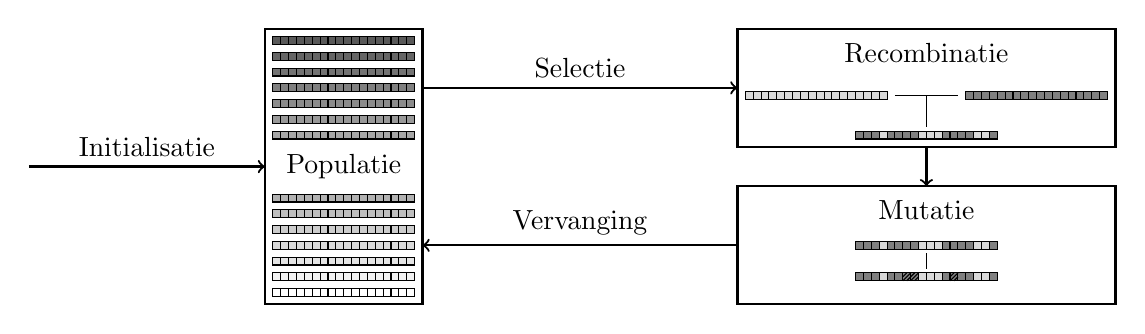
\begin{tikzpicture}
\draw[thick] (-1,-1.75) rectangle (1,1.75);
\draw (0,0) node {Populatie};
\foreach\y/\c/\d in {-1.65/0/65,-1.45/5/60,-1.25/10/55,-1.05/15/50,-0.85/20/45,-0.65/25/40,-0.45/30/35} {
  \filldraw[draw=black,fill=black!\c] (-0.9,\y) rectangle ++(1.8,0.1);
  \filldraw[draw=black,fill=black!\d] (-0.9,-\y) rectangle ++(1.8,-0.1);
  \foreach\x in {-0.8,-0.7,...,0.85} {
    \draw (\x,\y) -- ++(0,0.1);
    \draw (\x,-\y) -- ++(0,-0.1);
  }
}
\draw[thick,->] (-4,0) to node[midway,above]{Initialisatie} (-1,0);
\draw[thick,->] (1,1) to node[midway,above]{Selectie} (5,1);
\draw[thick] (5,0.25) rectangle ++(4.8,1.5);
\draw (7.4,1.45) node {Recombinatie};
\filldraw[draw=black,fill=black!15] (5.1,0.85) rectangle ++(1.8,0.1);
\filldraw[draw=black,fill=black!50] (7.9,0.85) rectangle ++(1.8,0.1);
\draw (7,0.9) -- (7.8,0.9);
\draw (7.4,0.9) -- (7.4,0.5);
\foreach\o/\n in {3/1,8/3,15/2} {
  \fill[black!15] (6.5+0.1*\o,0.35) rectangle ++(0.1*\n,0.1);
}
\foreach\o/\n in {0/3,4/4,11/4,17/1} {
  \fill[black!50] (6.5+0.1*\o,0.35) rectangle ++(0.1*\n,0.1);
}
\draw[black] (6.5,0.35) rectangle ++(1.8,0.1);
\foreach\x in {-0.8,-0.7,...,0.85} {
  \draw (6+\x,0.85) -- ++(0,0.1);
  \draw (8.8+\x,0.85) -- ++(0,0.1);
  \draw (7.4+\x,0.35) -- ++(0,0.1);
}
\draw[thick,->] (7.4,0.25) -- (7.4,-0.25);
\draw[thick] (5,-1.75) rectangle ++(4.8,1.5);
\draw (7.4,-0.55) node {Mutatie};
\draw (7.4,-1.1) -- (7.4,-1.3);
\foreach\o/\n in {3/1,8/3,15/2} {
  \fill[black!15] (6.5+0.1*\o,-1.05) rectangle ++(0.1*\n,0.1);
  \fill[black!15] (6.5+0.1*\o,-1.45) rectangle ++(0.1*\n,0.1);
}
\foreach\o/\n in {0/3,4/4,11/4,17/1} {
  \fill[black!50] (6.5+0.1*\o,-1.05) rectangle ++(0.1*\n,0.1);
  \fill[black!50] (6.5+0.1*\o,-1.45) rectangle ++(0.1*\n,0.1);
}
\foreach\o in {6,7,12} {
  \draw (6.5+0.1*\o,-1.45) -- (6.6+0.1*\o,-1.35);
  \draw (6.55+0.1*\o,-1.45) -- (6.6+0.1*\o,-1.4);
  \draw (6.5+0.1*\o,-1.4) -- (6.55+0.1*\o,-1.35);
}
\draw[black] (6.5,-1.05) rectangle ++(1.8,0.1);
\draw[black] (6.5,-1.45) rectangle ++(1.8,0.1);
\foreach\x in {-0.8,-0.7,...,0.85} {
  \draw (7.4+\x,-1.05) -- ++(0,0.1);
  \draw (7.4+\x,-1.45) -- ++(0,0.1);
}
\draw[thick,->] (5,-1) to node[midway,above]{Vervanging} (1,-1);
\end{tikzpicture}
\caption{Concept van genetische algoritmen.}
\label{fig:geneticAlgorithmsConcept}
\end{figure}
\subsubsection{Initialisatie} Bij de \termen{Initialisatie}-stap crieëren we een set van verschillende oplossingen, die we de \termen{populatie} of \termen{population} noemen. Deze populatie wordt meestal per toeval gegenereerd. Anderzijds kan deze uiteraard gegenereerd worden op basis van probleemkennis.
\subsubsection{Evaluatie}Vervolgens evalueren we in de \termen{Evaluatie}-stap alle individuen in de populatie. Dit doen we hoofdzakelijk op basis van hun utility-waarde. Deze wordt ook wel \termen{fitness value} genoemd.
\subsubsection{Selectie}Uit de populatie kiezen we in de \termen{Selectie} enkele goede oplossingen. Hierbij hoeven we echter niet per definitie de beste individuen te selecteren. Soms is het beter, om nog een extra toevalscomponent te laten spelen, waardoor we soms gewoon een goede kandidaat uitkiezen.
\subsubsection{Recombinatie}De kandidaten die we uit de populatie gekozen hebben, zullen we vervolgens \termen{recombineren}. Hierbij crieëren we nieuwe oplossingen uit twee bestaande oplossingen, door karakteristieken uit de twee DNA's te combineren, en daaruit nieuwe DNA's te bouwen.
\paragraph{}
Hoe worden twee bit-lijsten nu concreet gecombineerd? Meestal wordt hiervoor een techniek gebruikt die we \termen{Crossover} noemen. Hierbij hebben we vooraf bepaalde punten bepaald, \termen{$k$-points} genoemd, waarbij we de bron veranderen. Afwisselend tussen deze punten levert ofwel de ene ofwel de andere ouder de code voor het kind. Meestal wordt hierbij een ander kind gegenereerd, die bij ieder stuk de code van de ouder andere krijgt. Deze techniek is bovendien uitbreidbaar zodat een kind meer dan twee ouders kan hebben. Een andere methode die ook wel eens gehanteerd wordt is dat bij iedere bit elke ouder 50\% kans maakt om deze te leveren. Bij een nog andere methode overlopen we de bitlijst, en bij een zekere kans beschouwen we een Crossover.
\subsubsection{Mutatie}Meestal wordt er enige \termen{mutatie} toegepast op de nieuwe kinderen. Hierbij wordt het DNA door middel van toeval licht gewijzigd. Dit heeft meestal tot doel om bij populaties die erg monotoon zijn toch de nodige ``inspiratie'' te genereren.
\paragraph{}Indien alle ouders op eenzelfde bit dezelfde waarde hebben, zal deze bit bij het kind ook deze waarde krijgen. Het probleem is echter dat indien het grootste (en vooral beste) deel van de populatie deze waarde deelt, we op den duur deze waarde niet meer kunnen veranderen. Dit kan resulteren in het feit dat we een collectie aan slechte oplossingen onderzoeken. Een oplossing voor dit probleem is om sommige bits van de gegenereerde kinderen te doen veranderen. Een zogenoemde \termen{flipover}. Dit doen we door iedere bit te overlopen en indien een toevallig gegenereerd getal aan een bepaalde conditie voldoet (onder een zeer kleine kans), veranderen we de waarde van deze bit naar het omgekeerde.
\subsubsection{Vervanging}In de \termen{vervanging}sfase worden de kinderen in de populatie opgenomen, meestal worden er vervolgens individuen uit de populatie gezet, zodat de populatie niet al te groot wordt. Het verwijderen van individuen gebeurt opnieuw meestal op basis van de fitness-waarde. Maar ook hier weer hoeft dit geen deterministisch proces te zijn. Nadat een nieuwe generatie oplossingen in de populatie is opgenomen, beginnen we opnieuw met de evaluatie, en begint de lus opnieuw. Tijdens de uitvoer van het algoritme wordt meestal de tot dan toe beste oplossing telkens bijgehouden. Na een aantal maal het hele proces herhaald te hebben. Wordt dit resultaat vervolgens teruggegeven als eindoplossing.
\paragraph{}In de praktijk worden er zo'n drietal vervangingsstrategieën gebruikt:
\begin{itemize}
 \item \termen{Delete All} We verwijderen de volledige populatie, en voegen de niewe kinderen toe als nieuwe populatie.
 \item \termen{Steady-State} Hierbij verwijderen we telkens $n$ oude leden uit de populatie, de criteria hier voor zijn opnieuw zelf in te stellen (ouders, slechtste, beste,...) en voegen de nieuwe kinderen toe.
 \item \termen{Steady-State No Duplicates} Soms kunnen gegenereerde kinderen kopieën zijn van reeds bestaande individuen, in dat geval stijgt de kans op selectie, wat eventueel de evolutie van de populatie kan ondermijnen (indien een bepaald individu succesvol is, riskeren we dat na enige tijd de hele populatie uit dat individu bestaat). Hierbij worden dus de duplicaten verwijdert.
\end{itemize}
\subsubsection{Bemerkingen}Genetische Algoritmes zijn vooral geschikt voor \termen{sheduling} (het opstellen van planningen). Maar ze convergeren gegarandeert naar de meest optimale oplossing voor ieder probleem. Meestal wordt een genetisch algoritme hierbij niet alleen toegepast maar wordt het gecombineerd met een ander techniek zoals bijvoorbeeld Local Search. Dit produceert in het algemeen betere resultaten. In dat geval spreken we van \termen{Memetic Algorithms}.
\paragraph{Parameters}Parameters die we meestal zelf kunnen kiezen bij genetische algoritmes zijn:
\begin{itemize}
 \item De grootte van de populatie
 \item Kans op mutatie
 \item Crossover: $k$-punten of de kansen op een crossover.
\end{itemize}
Deze parameters worden meestal bepaald door experimenten op test-data (waarbij deze parameters vaak toevallig gezet worden, en de resultaten met andere vergeleken worden), in dat geval zijn ze statisch. Soms zijn ze echter dynamisch, en zal het algoritme ze zelf aanpassen, indien de gebruiker bijvoorbeeld niet tevreden is.
\begin{leftbar}
Door de binaire lijst $b_i$ als het DNA voor een oplossing te nemen bekomen we een eenvoudige representatie. We vullen initieel de populatie door een collectie aan toevallige binaire lijsten te genereren. Oplossingen die niet aan de gewichtsvoorwaarde voldoen worden eenvoudigweg uit de oplossing verwijdert. Als selectie nemen we eenvoudigweg de utility-waarde van de knapzak. Dit kan eventueel aangevuld worden met een stochastisch element, waardoor ook niet optimale oplossingen kunnen geselecteerd worden. Als recombinatie wordt per element in de nieuwe binaire lijst voor 50\% van de gevallen de ene ouder en in het ander geval de andere ouder als bron gebruikt. Eventueel kunnen we dus ook meerdere kinderen uit dezelfde ouders genereren. Als mutatie zullen we een bit omdraaien in de lijst met een kans van 0.1\%. Oplossingen die niet aan de voorwaarden voldoen worden niet toegevoegd aan de populatie. Als vervangstrategie gebruiken we Steady-State.
\end{leftbar}
\subsection{Tabu Search}
\label{ss:tabuSearch}
Tabu Search is een techniek waarbij we ervan uitgaan dat oplossingen die dicht bij elkaar liggen, meestal ongeveer dezelfde Utility-factor bezitten. We zouden dus de ruimte van oplossingen als een landschap kunnen zien, waarbij goede oplossingen een heuvel voorstellen. Tabu Search probeert hierbij op zoek te gaan naar de top van de hoogste berg. Indien we dit met behulp van een heuristiek zouden oplossen (we nemen de richting waarin we het snelst stijgen) dreigen we echter al snel op een lokaal maximum te stuiten. Een plaats waarbij alle dichte oplossingen slechter zijn, maar waarbij de eigen oplossing niet de beste is. Ook Simulated Annealing (zie \ref{ss:simulatedAnnealing}) werkt op basis van hetzelfde principe.
\paragraph{}De oplossing die Tabu Search biedt, is gebaseerd op het principe van \termen{tuning}. We bekijken nu een oplossing als een lijst van parameters (uiteraard kunnen we voor iedere parameter een bit nemen, en bekomen we opnieuw een lijst van bits). we zorgen er voor dat onze initiële oplossing aan alle constraints voldoet, vervolgens passen we een bepaalde parameter aan zodat we een nieuwe geldige toestand bekomen. Deze parameter wordt vervolgens in een lijst opgenomen, de \termen{Tabu List}. Dit is een lijst van parameters (en dus bewegingen in de oplossing) die tijdelijk niet mogen veranderen. Bij de volgende keuze van de parameter, mogen we alle parameters kiezen behalve deze in de Tabu List. Uiteraard worden de Tabu parameters na enige tijd weer verwijdert uit de lijst. Meestal heeft de lijst een vaste grootte die meestal vastgelegd wordt op een bepaalde factor van het aantal parameters. Bij de keuze welke parameters de lijst mogen verlaten indien de lijst overloopt zijn er enkele technieken: De parameter die er het langst in zit (de lijst is in dat geval een Queue), of een toevallige parameter zijn hierbij de populairste keuzes. Figuur \ref{fig:tabuSearchConcept} vat het concept achter Tabu Search schematisch samen.
\begin{figure}[htb]
\centering
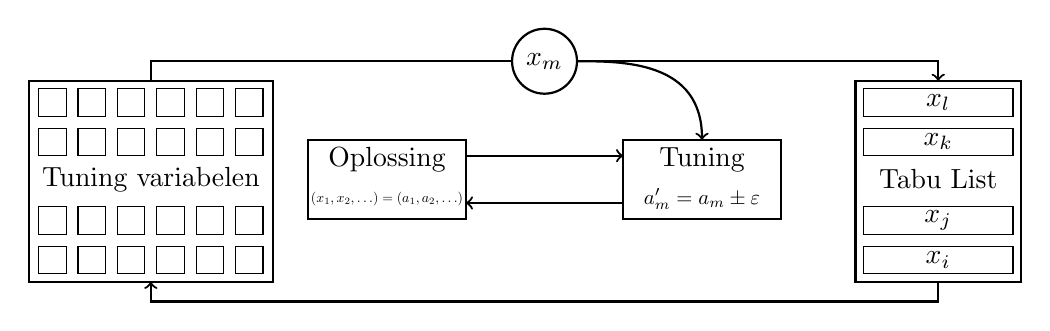
\begin{tikzpicture}
\draw[thick] (-1.05,-1.3) rectangle (1.05,1.25);
\draw (0,0) node {Tabu List};
\foreach\y/\t in {1/i,2/j,4/k,5/l} {
  \draw (-0.95,-1.7+0.5*\y) rectangle (0.95,-1.35+0.5*\y);
  \draw (0,-1.525+0.5*\y) node{$x_\t$};
}
\draw[thick] (-11.55,-1.3) rectangle (-8.45,1.25);
\draw (-10,0) node {Tuning variabelen};
\foreach\y in {1,2,4,5} {
  \foreach\x in {0,1,2,3,4,5} {
    \draw (-11.425+0.5*\x,-1.7+0.5*\y) rectangle ++(0.35,0.35);
  }
}
\draw[thick] (-8,-0.5) rectangle (-6,0.5);
\draw (-7,0.25) node {Oplossing};
\draw (-7,-0.25) node[scale=0.5] {$\left(x_1,x_2,\ldots\right)=\left(a_1,a_2,\ldots\right)$};
\draw (-3,-0.25) node[scale=0.75] {$a_m'=a_m\pm\varepsilon$};
\draw[thick] (-4,-0.5) rectangle (-2,0.5);
\draw (-3,0.25) node {Tuning};
\node[draw=black,circle,thick] (V) at (-5,1.5) {$x_m$};
\draw[thick,->] (-10,1.25) |- (V) -| (0,1.25);
\draw[thick,->] (0,-1.3) |- (-5,-1.55) -| (-10,-1.3);
\draw[thick,->] (-6,0.3) -- (-4,0.3);
\draw[thick,->] (-4,-0.3) -- (-6,-0.3);
\draw[thick,->] (V) .. controls ++(1,0) and (-3,1.5) .. (-3,0.5);
\end{tikzpicture}
\caption{Concept van Tabu Search.}
\label{fig:tabuSearchConcept}
\end{figure}
\subsubsection{Bemerkingen} Tabu Search is een techniek die vooral gebruikt wordt bij ruimteproblemen zoals het berekenen van de kortste route, het vullen van magazijnen,...
\begin{leftbar}
De implementatie van Tabu Search voor het knapzakprobleem is relatief eenvoudig. Als variabelen beschouwen we alle elementen uit de binaire rij. We zullen dus eenvoudigweg een willekeurig element omdraaien, en vervolgens de index hiervan aan de Tabu List toevoegen. Als grootte van de Tabu List nemen we bijvoorbeeld 10\% van de lengte van de binaire rij.
\end{leftbar}
\subsection{Simulated Annealing}
\label{ss:simulatedAnnealing}
Ook Simulated Annealing, ontwikkeld in 1983 door Kirkpatrick\footnote{Scott Kirkpatrick}, maakt gebruik van het dichte oplossings principe. Hierbij werd de inspiratie gehaald bij het stollen van kristallen. Kristallen verkrijgen bij een traag stollingsproces, de meest optimale geometrische structuur op atomair niveau. Dit effect probeert men met Simulated Annealing na te bootsen. Een kristal streeft immers naar een zo minimaal mogelijke potentiële energie. Hoewe we bij optimalisatie meestal op zoek zijn naar de maximale waarde, is het gebruik van een eenvoudig minteken voor de utility-functie, voldoende om van een optimaal minimum naar een optimaal maximum te gaan.
\paragraph{}De \termen{Vaste Stoffen Fysica} ofwel \termen{Solid State Physics} stelt dat de kans op een overgang tussen twee verschillende geometrieën $g_1$ en $g_2$ gekenmerkt wordt door volgende expressie:
\begin{equation}
P\left(g_1\rightarrow g_2\right)=\left\{\begin{array}{ll}
1&\mbox{if } U\left(g_2\right)\leq U\left(g_1\right)\\
e^{U\left(g_1\right)-U\left(g_2\right)/k_B\cdot T}&\mbox{otherwise}
\end{array}\right.
\end{equation}
De geometrieën zelf liggen over het algemeen niet ver uit elkaar (in de fysische wereld verschillen ze hoogstens enkele kwantum-niveaus). Verder is $U\left(g\right)$ de potentieële energie van een bepaalde geometrie $g$, $k_B$ is de Boltzmann constante en $T$ is de temperatuur in Kelvin op dat moment. We merken hierbij op dat indien we naar een energetisch lagere geometrie gaan de kans $P=1$, en dus bijgevolg deze transactie altijd ondersteund wordt. Indien we naar een hogere energetische waarde gaan is de kans eerder beperkt. Deze kans hangt dan ook grotendeels af van de heersende temperatuur: onder extreem hoge temperatuur worden alle overgangen nagenoeg toegestaan, bij zeer lage temperaturen zijn dergelijke overgangen quasi onmogelijk. Indien we de temperatuur maar traag genoeg doen zakken zal de geometrie bij iedere temperatuur een staat bereiken die we \termen{Thermal Equilibrium} noemen. Hierbij is de kansverdeling voor iedere mogelijke transitie gegeven door:
\begin{equation}
P\left(X=i\right)=\displaystyle\frac{e^{-U_i/k_B\cdot T}}{\sum_j e^{-U_j/k_B\cdot T}}
\end{equation}
Het \termen{Metropolis Algoritme} is een gekende generator van nieuwe staten in een problemen vertrekkende vanaf een bepaalde staat. Door dit concept toe te passen op een oplossingsverzameling bereiken we meestal zeer goede resultaten, indien we eerst onze staat naar een Thermisch Evenwicht laten convergeren kunnen we zelfs de meest optimale oplossing bereiken. Formeel kunnen we dit concept uitdrukken in \algref{alg:simulatedAnnealing}. Een conceptueel schema staat op figuur \ref{fig:simulatedAnnealingConcept}.
\begin{algorithm}[htb]
\caption{Simulated Annealing}
\label{alg:simulatedAnnealing}
\begin{algorithmic}[1]
\STATE $S\leftarrow S_{\mbox{start}}$\COMMENT{$S$ is de huidige oplossings-staat}
\STATE $c\leftarrow c_i$\COMMENT{zet de controle parameter op een initiele waarde}
\STATE $L\leftarrow L_i$\COMMENT{initiële herhalingslengte}
\WHILE{$c>c_f$}
\FOR{$l=1$ to $L$}
\STATE $S_j\leftarrow\mathcommand{generateNextRandomStep}{S}$
\IF{$\mathcommand{random}{0,1}<e^{f\left(S_j\right)-f\left(S\right)/c}$}
\STATE $S\leftarrow S_j$
\ENDIF
\ENDFOR
\STATE $c\leftarrow\mathcommand{changeControl}{c}$
\STATE $L\leftarrow\mathcommand{changeLength}{L}$
\ENDWHILE
\end{algorithmic}
\end{algorithm}
Hierbij is $c$ een controleparameter die we fysisch kunnen zien als $k_B\cdot T$.
\begin{figure}[htb]
\centering
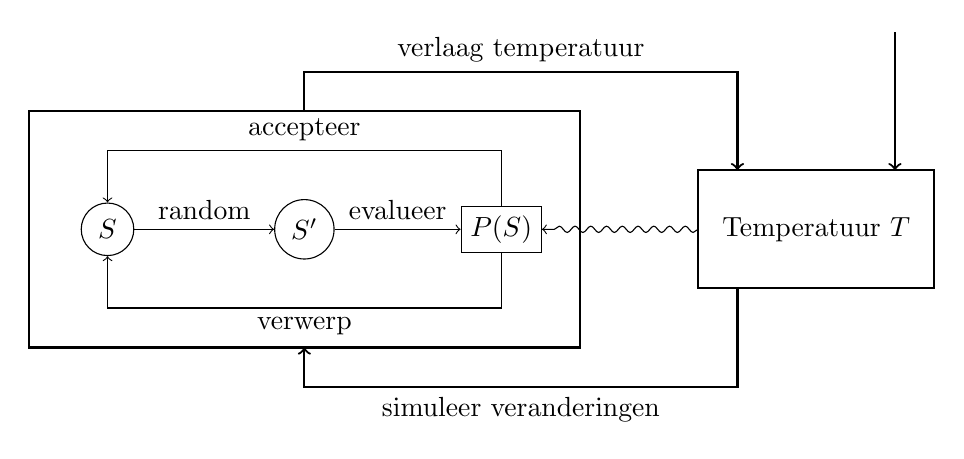
\begin{tikzpicture}
\draw[thick] (5,-0.75) rectangle (8,0.75);
\draw (6.5,0) node {Temperatuur $T$};
\draw[thick] (-3.5,-1.5) rectangle (3.5,1.5);
\node[draw=black,circle] (S1) at (-2.5,0) {$S$};
\node[draw=black,circle] (S2) at (0,0) {$S'$};
\node[draw=black,rectangle] (P) at (2.5,0) {$P(S)$};
\draw[->] (S1) to node[midway,sloped,above]{random} (S2);
\draw[->] (S2) to node[midway,sloped,above]{evalueer} (P);
\draw[->] (P.south) -- (2.5,-1) to node[below,midway,sloped] {verwerp} (-2.5,-1) -- (S1);
\draw[->] (P.north) -- (2.5,1) to node[above,midway,sloped] {accepteer} (-2.5,1) -- (S1);
\draw[->,decorate,decoration={snake,amplitude=.4mm,segment length=2mm,post length=1mm}] (5,0) -- (P);
\draw[thick,->] (7.5,2.5) -- (7.5,0.75);
\draw[thick,->] (0,1.5) -- (0,2) to node[midway,sloped,above]{verlaag temperatuur} (5.5,2) -- (5.5,0.75);
\draw[thick,->] (5.5,-0.75) -- (5.5,-2) to node[midway,sloped,below]{simuleer veranderingen} (0,-2) -- (0,-1.5);
\end{tikzpicture}
\caption{Concept van Simulated Annealing.}
\label{fig:simulatedAnnealingConcept}
\end{figure}
\subsubsection{Bemerkingen}
Simulated Annealing is een techniek die vooral intressant is bij problemen met grafen (kleuren van grafen) en sheduling. Daarintegen blijkt Simulated Annealing niet echt geschikt te zijn voor problemen zoals het Handelsreizigersprobleem. In de praktijk wordt het dan ook bijvoorbeeld gebruikt voor Image Processing. Hierbij werkt het meestal beter dan tijdsequivalente methodes, en ondergaat het minder problemen wanneer de grootte van het probleem opgedreven wordt. Een probleem is echter dat de kwaliteit van belangrijke factoren zoals het regelen van de temperatuur, en het bepalen van wat dichte oplossingen zijn, hoofdzakelijk bepaald worden door de vaardigheden van de programmeur. Een foute keuze kan tot zeer slechte resultaten leiden.
\begin{leftbar}
We gaan van een toestand in een andere door een object toe te voegen aan onze knapzak, en indien hierbij de gewichtvoorwaarde geschonden wordt toevallige objecten uit de knapzak te halen tot het gewicht weer klopt. Als begintemperatuur stellen we bijvoorbeeld $300\mbox{ K}$ in. Per temperatuur zullen we 25 keer van configuratie veranderen. Vervolgens vermenigvuldigen we de temperatuur met $0.9$. We laten het algoritme stoppen indien de temperatuur onder de $1\mbox{ K}$. In totaal zullen we dus $1375$ van toestand proberen te veranderen.
\end{leftbar}
\subsection{Variable Neighbourhood Search}
\label{ss:variableNeighbourhoodSearch}
Net als Tabu Search en en Simulated Annealing beroept ook Variable Neighbourhood Search zich op het lokaliteitsprincipe. Het stelt dus dat goede oplossingen meestal in de buurt liggen van elkaar. Om echter het probleem met lokale maxima op te lossen, probeert men niet het algoritme te dwingen naar alternatieven te kijken, het stelt gewoon de op dat moment geldende definitie van buurt (lokaliteit) in vraag. Indien we deze definitie veranderen kunnen twee oplossingen die eerst dicht bij elkaar lagen, ineens geen echte band meer hebben. Indien we dus op een lokaal maximum botsen, kunnen we eenvoudigweg door de definitie om te vormen een nieuw landschap bouwen waar het uiteindelijk de bedoeling is om de hoogste berg te beklimmen. Bij iedere definitie zoeken we telkens naar de beste buur, dit proces wordt \termen{Exploring} genoemd. Het algoritme is formeel te beschreven in \algref{alg:variableNeighbourhoodSearch}.
\begin{algorithm}[htb]
\caption{Variable Neighbourhood Search}
\label{alg:variableNeighbourhoodSearch}
\begin{algorithmic}[1]
\STATE $\mathfrak{H}\leftarrow$\COMMENT{Set van neighbourhood structuren}
\STATE $x\leftarrow x_0$\COMMENT{Initiele oplossing}
\STATE $l\leftarrow 0$
\WHILE{$l<\#\mathfrak{H}$}
\STATE $x'\leftarrow\mathcommand{bestNeighbourByStructure}{x,\mathfrak{H}\left[l\right]}$
\IF{$\mathcommand{utility}{x'}>\mathcommand{utility}{x}$}
\STATE $l\leftarrow 0$
\STATE $x\leftarrow x'$
\ELSE
\STATE $l\leftarrow l+1$
\ENDIF
\ENDWHILE
\end{algorithmic}
\end{algorithm}
Meestal ordent men hier de neighbourhood definties zodaning dat de eerst een kleine regio rond de huidige oplossing onderzoekt, en dus snel tot een resultaat komt. De laatste definitie zoekt daarintegen meestal een zeer groot gebied af. Verder wordt dit algoritme meestal herhaalt in een extra lus die pas stopt indien aan een bepaald terminatiecriterium voldaan is. Naast het zonet beschreven algoritme bestaan er heel wat varianten van Variable Neighbourhood Search, de belangrijkste sommen we hieronder op. Het algemene concept van Variable Neighbourhood Search wordt geschematiseerd in figuur \ref{fig:variableNeighbourhoodSearchConcept}.
\begin{figure}[htb]
\centering
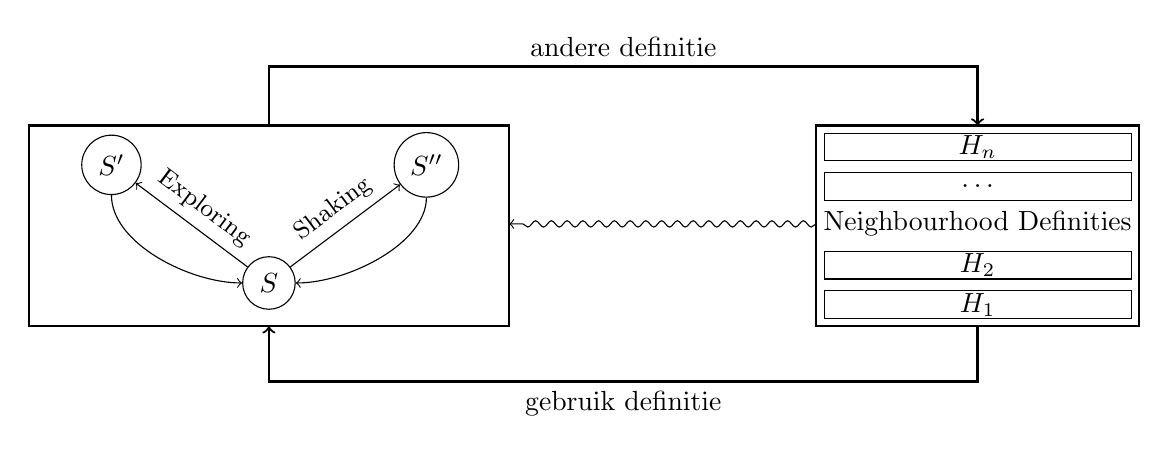
\begin{tikzpicture}
\draw[thick] (-2.05,-1.3) rectangle (2.05,1.25);
\draw (0,0) node {Neighbourhood Definities};
\foreach\y/\t in {1/\mathfrak{H}_1,2/\mathfrak{H}_2,4/\ldots,5/\mathfrak{H}_n} {
  \draw (-1.95,-1.7+0.5*\y) rectangle (1.95,-1.35+0.5*\y);
  \draw (0,-1.525+0.5*\y) node{$\t$};
}
\draw[thick] (-12.05,-1.3) rectangle (-5.95,1.25);
\node[draw=black,circle] (S) at (-9,-0.75) {$S$};
\node[draw=black,circle] (S1) at (-11,0.75) {$S'$};
\node[draw=black,circle] (S2) at (-7,0.75) {$S''$};
\draw[->] (S) to node[sloped,midway,above]{\small{Exploring}} (S1);
\draw[->] (S) to node[sloped,midway,above]{\small{Shaking}} (S2);
\draw[->] (S1) .. controls ++(0,-1) and (-10,-0.75) .. (S);
\draw[->] (S2) .. controls ++(0,-1) and (-8,-0.75) .. (S);
\draw[->,decorate,decoration={snake,amplitude=.4mm,segment length=2mm,post length=1mm}] (-2.05,0) -- (-5.95,0);
\draw[->,thick] (0,-1.3) -- (0,-2) to node[midway,sloped,below]{gebruik definitie} (-9,-2) -- (-9,-1.3);
\draw[->,thick] (-9,1.25) -- (-9,2) to node[midway,sloped,above]{andere definitie} (0,2) -- (0,1.25);
\end{tikzpicture}
\caption{Concept van Variable Neighbourhood Search.}
\label{fig:variableNeighbourhoodSearchConcept}
\end{figure}
\subsubsection{Variable Neighbourhood Search Reduced}
\termen{Variable Neighbourhood Search Reduced} is een snellere variant. Hierbij wordt niet gezocht naar de beste buur, maar kiezen we gewoon een toevallige buur. Het generen van een toevallige buur wordt \termen{Shaking} genoemd. Alsof een beving in het landschap ons naar dichtbij gelegen punt brengt. Uiteraard leidt dit er toe dat we vaker van Neighbourhood Structure moeten wisselen. Anderzijds kan het generen van een random buur meestal in \bigoh{1} gedaan worden, terwijl het zoeken naar de beste buur \bigoh{n} vereist (waarbij $n$ zeer groot kan zijn). Dit algoritme komt meestal tot een minder goede oplossing, maar werkt meestal opvallend sneller. Bovendien kan het resultaat die we hier mee bereikt hebben opnieuw ingegeven worden in een andere implementatie van Variable Neighbourhood Search die de oplossing verder optimaliseert. Dit algoritme wordt beschreven in \algref{alg:variableNeighbourhoodSearchReduced}.
\begin{algorithm}[htb]
\caption{Variable Neighbourhood Search Reduced}
\label{alg:variableNeighbourhoodSearchReduced}
\begin{algorithmic}[1]
\STATE $\mathfrak{H}\leftarrow$\COMMENT{Set van neighbourhood structuren}
\STATE $x\leftarrow$\COMMENT{Initiele oplossing}
\STATE $l\leftarrow 0$
\WHILE{$l<\#\mathfrak{H}$}
\STATE $x'\leftarrow\mathcommand{randomNeighbourByStructure}{x,\mathfrak{H}\left[l\right]}$
\IF{$\mathcommand{utility}{x'}>\mathcommand{utility}{x}$}
\STATE $l\leftarrow 0$
\STATE $x\leftarrow x'$
\ELSE
\STATE $l\leftarrow l+1$
\ENDIF
\ENDWHILE
\end{algorithmic}
\end{algorithm}
\subsubsection{Variable Neighbourhood Search Basic}
\termen{Variable Neighbourhood Search Basic} is een combinatie van Variable Neighbourhood Search en Variable Neighbourhood Search Reduced. Hierbij genereren we een toevallige buur, waarna we vanuit deze buur een beste buur zoeken. Deze tweede buur wordt dan vervolgens geëvalueerd en verworpen of aangenomen. Dit staat beschreven in \algref{alg:variableNeighbourhoodSearchBasic}.
\begin{algorithm}[htb]
\caption{Variable Neighbourhood Search Basic}
\label{alg:variableNeighbourhoodSearchBasic}
\begin{algorithmic}[1]
\STATE $\mathfrak{H}\leftarrow$\COMMENT{Set van neighbourhood structuren}
\STATE $x\leftarrow$\COMMENT{Initiele oplossing}
\STATE $l\leftarrow 0$
\WHILE{$l<\#\mathfrak{H}$}
\STATE $x'\leftarrow\mathcommand{randomNeighbourByStructure}{x,\mathfrak{H}\left[l\right]}$
\STATE $x''\leftarrow\mathcommand{bestNeighbourByStructure}{x',\mathfrak{H}\left[l\right]}$
\IF{$\mathcommand{utility}{x''}>\mathcommand{utility}{x}$}
\STATE $l\leftarrow 0$
\STATE $x\leftarrow x''$
\ELSE
\STATE $l\leftarrow l+1$
\ENDIF
\ENDWHILE
\end{algorithmic}
\end{algorithm}
\subsubsection{Variable Neighbourhood Search General}
Een implementatie van Variable Neighbourhood Search waarij we blijven zoeken tot we $k_{\mbox{max}}$ keer geen verbetering zien optreden heet \termen{Variable Neighbourhood Search General}. Deze implementatie kan in sommige gevallen zelfs ertoe leiden dat men de omhullende lus die het uiteindelijke stopcriterium bepaald, weglaat. Indien $k_{\mbox{max}}$ goed gekozen is (te klein levert een slechte oplossing, te groot zorgt voor de nodige overhead), kan dit algoritme in de meeste gevallen het meeste efficiënt met zijn tijd omspringen. Omdat naast de Neighbourhood Structuren we alleen maar een parameter $k_{\mbox{max}}$ nodig hebben, kan deze parameter vaak eenvoudig door testdata bepaald worden. \algref{alg:variableNeighbourhoodSearchGeneral} beschrijft dit concept formeel.
\begin{algorithm}[htb]
\caption{Variable Neighbourhood Search General}
\label{alg:variableNeighbourhoodSearchGeneral}
\begin{algorithmic}[1]
\STATE $\mathfrak{H}\leftarrow$\COMMENT{Set van neighbourhood structuren}
\STATE $x\leftarrow$\COMMENT{Initiele oplossing}
\STATE $l\leftarrow 0$
\STATE $k\leftarrow 0$
\WHILE{$k<k_{\mbox{max}}$}
\STATE $x'\leftarrow x$
\WHILE{$l<\#\mathfrak{H}$}
\STATE $x''\leftarrow\mathcommand{bestNeighbourByStructure}{x',\mathfrak{H}\left[l\right]}$
\IF{$\mathcommand{utility}{x''}>\mathcommand{utility}{x'}$}
\STATE $l\leftarrow 0$
\STATE $x'\leftarrow x''$
\ELSE
\STATE $l\leftarrow l+1$
\ENDIF
\ENDWHILE
\IF{$\mathcommand{utility}{x'}>\mathcommand{utility}{x}$}
\STATE $k\leftarrow 0$
\STATE $x\leftarrow x'$
\ELSE
\STATE $k\leftarrow k+1$
\ENDIF
\ENDWHILE
\end{algorithmic}
\end{algorithm}
\subsubsection{Bemerkingen}
Variable Neighbourhood Search is een techniek die vooral gespecialiseerd is in het oplossen van problemen in verband met grafen, sheduling en locatieproblemen.
\subsection{Hyperheuristics}
\label{ss:hyperheuristics}
De meeste heuristieken hebben slechts een specialisatie op een bepaald gebied. Dit leid er toe dat we eigenlijk nog steeds geen algemeen algoritme hebben. Hyperheuristics is een poging om tot een algoritme te komen die in principe alle problemen met een zekere optimaliteit kan oplossen. Hyperheuristics zelf is echter geen algoritme, het is een techniek die allerhande Metaheuristieken (zoals deze die in de vorige subsecties besproken werden) combineert, om zo telkens tot de optimale mix te komen. Hierbij definiëren we een set van Metaheuristieken die een bepaald probleem kunnen oplossen. Door deze Metaheuristieken op enkele testproblemen te laten lopen, komen we te weten hoe goed iedere Metaheuristiek presteert op het soort probleem dat we willen oplossen. Het komt er dan ook op neer dat we de heuristieken op de één of andere manier gaan combineren met elkaar. Volgens een bepaalde keuzefunctie kunnen we dan vervolgens selecteren hoe vaak we een bepaalde Metaheuristiek op het probleem loslaten, alvorens we een andere aan de beurt laten. Doormiddel van Machine Learning kunnen we deze keuzefunctie dan verbeteren, tot we een algoritme bekomen die over het algemeen een zeer optimale oplossing teruggeeft.
